\section{Analyse}
\label{sec:analyse}
Nachdem ein geeigneter Datensatz erfasst wurde, können die Daten analysiert werden.
Für die Analyse gibt es zwei wesentliche Herangehensweisen: Korrelationsmaße und Klassifikatoren.
Zuvor sollte festgelegt werden, welche Metriken für die Analyse verwendet werden sollen.
%TODO Medeiros et. al versuchen, die besten Metriken herauszufinden!
% Informational approach (Wo fließen Daten hin?) vs. structual approach (Wer ruft wen auf?)

\subsection{Wahl der Metriken}
Die Auswahl der Metriken ist vielfältig.
In \cite{alves_et_al} werden insgesamt 27 Metriken für Funktionen berechnet.
Einige davon sind CCC-Metriken\footnote{Die Metriken sind jedoch nicht in die Komplexität, Kopplung und Kohäsion eingeteilt.}, andere beziehen sich auf die Anzahl der Codezeilen oder auf das Verhältnis von Quellcode-Kommentaren zu Codezeilen.
In der Studie aus \cite{chowdhury_zulkernine_2009} werden 21 Metriken berechnet.
Die Forscher teilen dabei die Metriken sowohl in die CCC-Klassen, als auch in Code-Level und Design-Level ein.
Unter Design-Level-Metriken versteht man dabei solche, die nach dem Entwurf der Software (beispielsweise anhand eines UML-Klassendiagramms) berechnet werden können.
Implementierungsspezifische Metriken wie die Anzahl Code-Zeilen bezeichnen sich als Code-Level-Metriken.
Abbildung \ref{fig:chowdhury_metrics} zeigt einen Ausschnitt aus \cite{chowdhury_zulkernine_2010}.
Zu sehen sind die Bezeichnung und englische Beschreibungen für die Komplexitätsmetriken.
\begin{figure}
	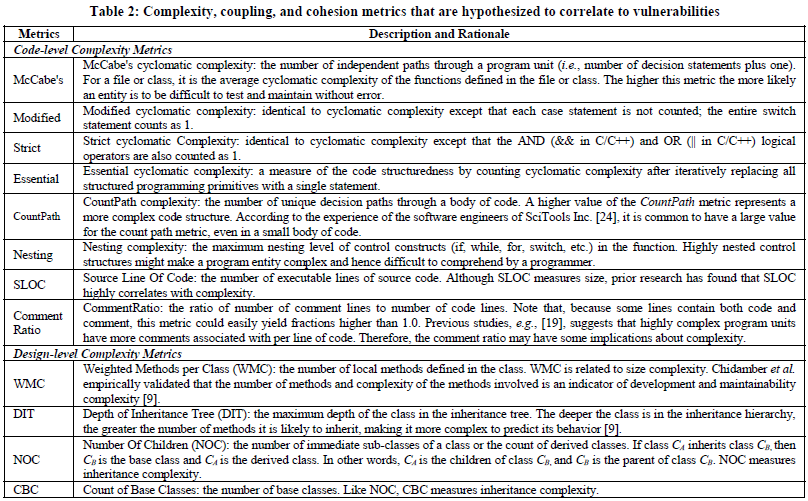
\includegraphics[width=\textwidth]{img/chowdhury_metrics.png}
	\caption{Auszug aus \cite{chowdhury_zulkernine_2010}; Tabelle mit den verwendeten Metriken.}
	\label{fig:chowdhury_metrics}
\end{figure}

\subsection{Korrelationsmaße}
Zur Überprüfung der Hypothesen eigen sich Korrelationsmaße.
Die Behebung einer Sicherheitslücke müsste eine Verbesserung der CCC-Metriken nach sich ziehen.
Ein mögliches Maß für die Korrelation ist Spearmans Rangkorrelationskoeffizient~\cite{alves_et_al,chowdhury_zulkernine_2010}, da dieses keine Annahmen zur Verteilung macht.
Der Spearman Korrelationskoeffizient (kurz: die Korrelation) ist ein Wert zwischen -1 und +1, wobei -1 eine stark negative und +1 eine stark positive Korrelation ausdrückt.
Die Signifikanz der Korrelation wird mit dem p-Wert ausgerückt.
Ein p-Wert kleiner 0.05 wird als statistisch signifikant gewertet.
Weitere Techniken, die beispielsweise in \cite{alves_et_al} verwendet werden, sind der zweiseitige t-Test, Konfidenzintervalle und der Wilcoxon Rangsummentest.
\begin{figure}
	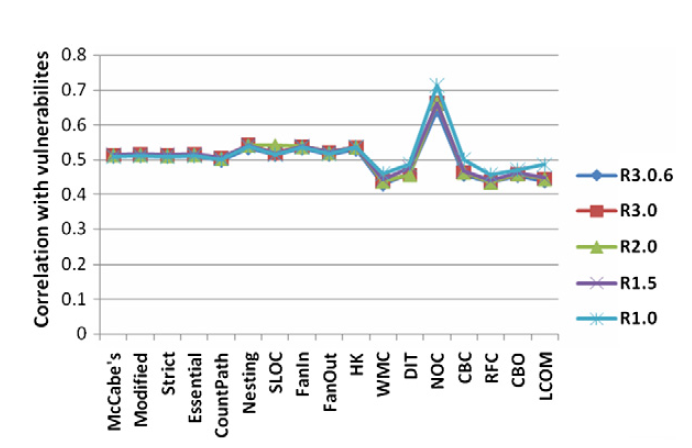
\includegraphics[width=\textwidth]{img/vulnerability_correlations.png}
	\caption{Korrelationen mit Sicherheitslücken zu verschiedenen Metriken}
	\label{fig:correlations}
\end{figure}
Abbildung \ref{fig:correlations} aus \cite{chowdhury_zulkernine_2009} zeigt die Korrelation mit Sicherheitslücken zu verschiedenen Metriken.
Die Linien zeigen verschiedene Release-Versionen von Mozilla Firefox.
Es lässt sich erkenne, dass die Korrelationsmuster über Versionen hinweg konsistent sind\cite{chowdhury_zulkernine_2009}.

\subsection{Klassifikatoren}
Mithilfe der Metriken lassen sich auch Klassifikatoren erstellen.
Dieser Ansatz wird in \cite{chowdhury_zulkernine_2009} verwendet, um ein Framework für die Vorhersage von Sicherheitslücken zu entwickeln.
Die Herangehensweise unterscheidet sich dahingehend von der Berechnung der Korrelationen, dass die in anderen Studien festgestellte Korrelation der Metriken mit Sicherheitslücken nicht verwendet wurde, um Vorhersagen zu erstellen.

Das Problem wird als Klassifizierungsproblem auf Dateiebene aufgefasst:
Entweder eine Datei ist anfällig für Sicherheitslücken oder nicht.
Für die Klassifikatoren kommen verschiedene Techniken in Frage.
Beispiele sind \emph{C4.5 Entscheidungsbäume}\cite{decision_trees}, die Weiterentwicklung \emph{Random Forests} und der \emph{Bayes-Klassifikator}.
